%Copyright 2014 Jean-Philippe Eisenbarth
%This program is free software: you can 
%redistribute it and/or modify it under the terms of the GNU General Public 
%License as published by the Free Software Foundation, either version 3 of the 
%License, or (at your option) any later version.
%This program is distributed in the hope that it will be useful,but WITHOUT ANY 
%WARRANTY; without even the implied warranty of MERCHANTABILITY or FITNESS FOR A 
%PARTICULAR PURPOSE. See the GNU General Public License for more details.
%You should have received a copy of the GNU General Public License along with 
%this program.  If not, see <http://www.gnu.org/licenses/>.

%Based on the code of Yiannis Lazarides
%http://tex.stackexchange.com/questions/42602/software-requirements-specification-with-latex
%http://tex.stackexchange.com/users/963/yiannis-lazarides
%Also based on the template of Karl E. Wiegers
%http://www.se.rit.edu/~emad/teaching/slides/srs_template_sep14.pdf
%http://karlwiegers.com


\documentclass{scrreprt}
\usepackage{listings}
\usepackage{underscore}
\usepackage[bookmarks=true]{hyperref}
\usepackage[utf8]{inputenc}
\usepackage[english]{babel}
\usepackage{pgf}
\usepackage{float}
\usepackage{graphicx,wrapfig}

\hypersetup{
    bookmarks=false,    % show bookmarks bar?
    pdftitle={Software Requirement Specification},    % title
    pdfauthor={Jean-Philippe Eisenbarth},                     % author
    pdfsubject={TeX and LaTeX},                        % subject of the document
    pdfkeywords={TeX, LaTeX, graphics, images}, % list of keywords
    colorlinks=true,       % false: boxed links; true: colored links
    linkcolor=blue,       % color of internal links
    citecolor=black,       % color of links to bibliography
    filecolor=black,        % color of file links
    urlcolor=purple,        % color of external links
    linktoc=page            % only page is linked
}%
\def\myversion{1.0 }
\date{}
%\title
\usepackage{hyperref}
\begin{document}

\begin{flushright}
    \rule{16cm}{5pt}\vskip1cm
    \begin{bfseries}
        \LARGE{SOFTWARE REQUIREMENTS\\ SPECIFICATION}\\
		\vspace{1cm}
		\LARGE{SOFTWARE DESIGN DESCRIPTION}\\
        \vspace{1cm}
        for\\
        \vspace{1cm}
		A WEB-BASED PROTOTYPE FOR REMOTE CAR DIAGNOSTICS\\
        \vspace{1cm}
        \Large{Version \myversion approved}\\
        \vspace{1cm}
        Prepared by\\
        \vspace{0.5cm} 
        Bogdan Lupu\\
        Ciprian Mierea\\
        Iulia Lazaroae\\
        Dragos Duca\\
        \vspace{1cm}
        MOBU\\
        \vspace{1cm}
        \today\\
    \end{bfseries}
\end{flushright}

\tableofcontents


\chapter*{Revision History}

\begin{center}
    \begin{tabular}{|c|c|c|c|}
        \hline
	    Name & Date & Reason For Changes & Version\\
        \hline
	    Bogdan Lupu & 13.09 & Initial Version of Document  & 0.0.1\\
        \hline
	    Bogdan Lupu & 13.09 & Add use cases & 0.0.1\\
        \hline
        Duca Dragos & 14.09 & Add add requirements & 0.0.1\\
        \hline
         Iulia Lazaroae & 14.09 & fill external interface requirements & 0.0.1\\
        \hline
        Mierea Ciprian & 14.09 & Filled in some Missing Sections & 0.0.1\\
        \hline
        Bogdan Lupu & 15.09 & Final state & 1.0.0\\
        \hline
    \end{tabular}
\end{center}

\part{About this document}
\chapter{Introduction}
This document implements the Software Architectural Design Description.
This document provides:
\begin{enumerate}
    \item the purpose or role in the system.
    \item the major goals.
    \item the connections to other components in the system.
    \item boundaries and limitations.
    \item relations with the outside world.
    \item major technical assumptions and constraints.
    \item the requirements or analysis regarding:
    \begin{itemize}
        \item stability: how is it ensured that other components do not 
                    compromise the stability of the described component.
        \item reliability: that in case of a failure, how the described 
                    component can return to normal operation without data loss.
        \item security: that the described component takes necessary security measurements into account.
        \item extensibility: that the component can be extended and/or tailored to upcoming needs.
        \item performance: that the component is capable to fulfill the performance requirements.
        \item reporting: that it is possible to monitor/analyze the operation of the component.
    \end{itemize}
\end{enumerate}

\part{Software Requirement Specification}
\chapter{Introduction}

\section{Purpose}
This document includes software requirements for Remote Diagnostics,
release number 1.0. Remote Diagnostics is licensed under the MIT License (MIT).
The system gives resolution to the remote car diagnostic problem.
It's purpose is to provide a way to share the malfunctions detected
by the car sensors with a car technician in order to get assistance.
Besides this functionality, the system is cross-platform which means
it can run directly on any operating system without additional preparation


\section{Document Conventions}
This document follows MLA Format. Bold-faced text has been used to emphasize section
and sub-section headings. Highlighting is to point out words in the glossary and italicized text is
used to label and recognize diagrams.

\section{Intended Audience and Reading Suggestions}
The intended audience for this document is composed of the development team, the project managers,
the testers and the documentation writers.
Everyone else may review the document to learn about this project and to understand the requirements.
The intended audience needs to become intimately familiar with the SRS.

\section{Project Scope}
The Remote Diagnostics has features that allow any person that owns a car with the Remote Diagnostic system
to share the malfunctions reported by the car's sensors with a car technician or any auto repair service in order
to get professional aid. Besides this functionality, the system is cross-platform which means
it can run directly on any operating system without additional preparation thus eliminating the need of specialized
software, hardware and reducing the cost of such solutions. Refer to the project scope document for further information.


\chapter{Overall Description}

\section{Product Perspective}
Remote Diagnostics is a product which targets to replace old-fashioned car diagnostic systems
for various reasons.
Performing a car diagnostic can reveal a number of problems associated with the transmission,
oil tank, gas tank, exhaust system and other components of the vehicle and all this information
can help the mechanic or the car dealership to fix the car issues faster and even prevent them from
happening.
This sounds all good until you look at the costs of those old-fashioned car diagnostic systems (example: handheld scanner devices)
Remote Diagnostics solves this problem hence it is mainly developed using web technologies (js, html, css) and gathers the infomation
provided by an OBD data logger.



\section{Product Functions}
\begin{itemize}
\item The user can retrieve sensor information from ODB by pressing a button
\item The user can easily send this information to his car mechanic / car dealership
\item As an added bonus, the user has limited car controlling features available through the product
\end{itemize}

\section{Operating Environment}
The preffered operating environment is composed of a linux webserver (RHEL7.1)
with NodeJS(latest stable version),ExpressJS(latest stable version) and MongoDB (latest version) installed.
Any other operating system capable of supporting NodeJS, ExpressJS and MongoDB should do but we don't guarantee it.


\section{Design and Implementation Constraints}
\begin{itemize}
\item As the system relies on JS heavily it will not operate on non-js compatible browsers.
\item JS is not very mature in the automotive domain.
\item The users needs to install the ODB logger on his own.
\item Everyone using this project has to read and agree with the MIT license.
\item The specific mentioned technologies in the Operating Environment section need to be used as specified.
\item The product's interface language is english.
\end{itemize}

\section{User Documentation}
The user documentation will be solely composed of a MediaWiki instance that will be updated with each software revision.
The wiki should include a pinned quick start article that shows how to setup and use the system.
No other user documentation should be provided.

\section{Assumptions and Dependencies}

\begin{itemize}
\item Internet is a must in order to share the data with a mechanic / car dealership
\item Using a browser that supports JS is a must to use the system at all
\item Users with old-cars that do not feature an ODB cannot use the system
\item It is assumed that the user knows how to use an internet browser.
\end{itemize}



\chapter{External Interface Requirements}

\section{User Interfaces}
Describe the logical characteristics of each interface between the software 
product and the users. This may include sample screen images, any GUI standards 
or product family style guides that are to be followed, screen layout 
constraints, standard buttons and functions (e.g., help) that will appear on 
every screen, keyboard shortcuts, error message display standards, and so on.  
Define the software components for which a user interface is needed. Details of 
the user interface design should be documented in a separate user interface 
specification.
\subsection{First Page}


\begin{figure}[!htbp]
\center
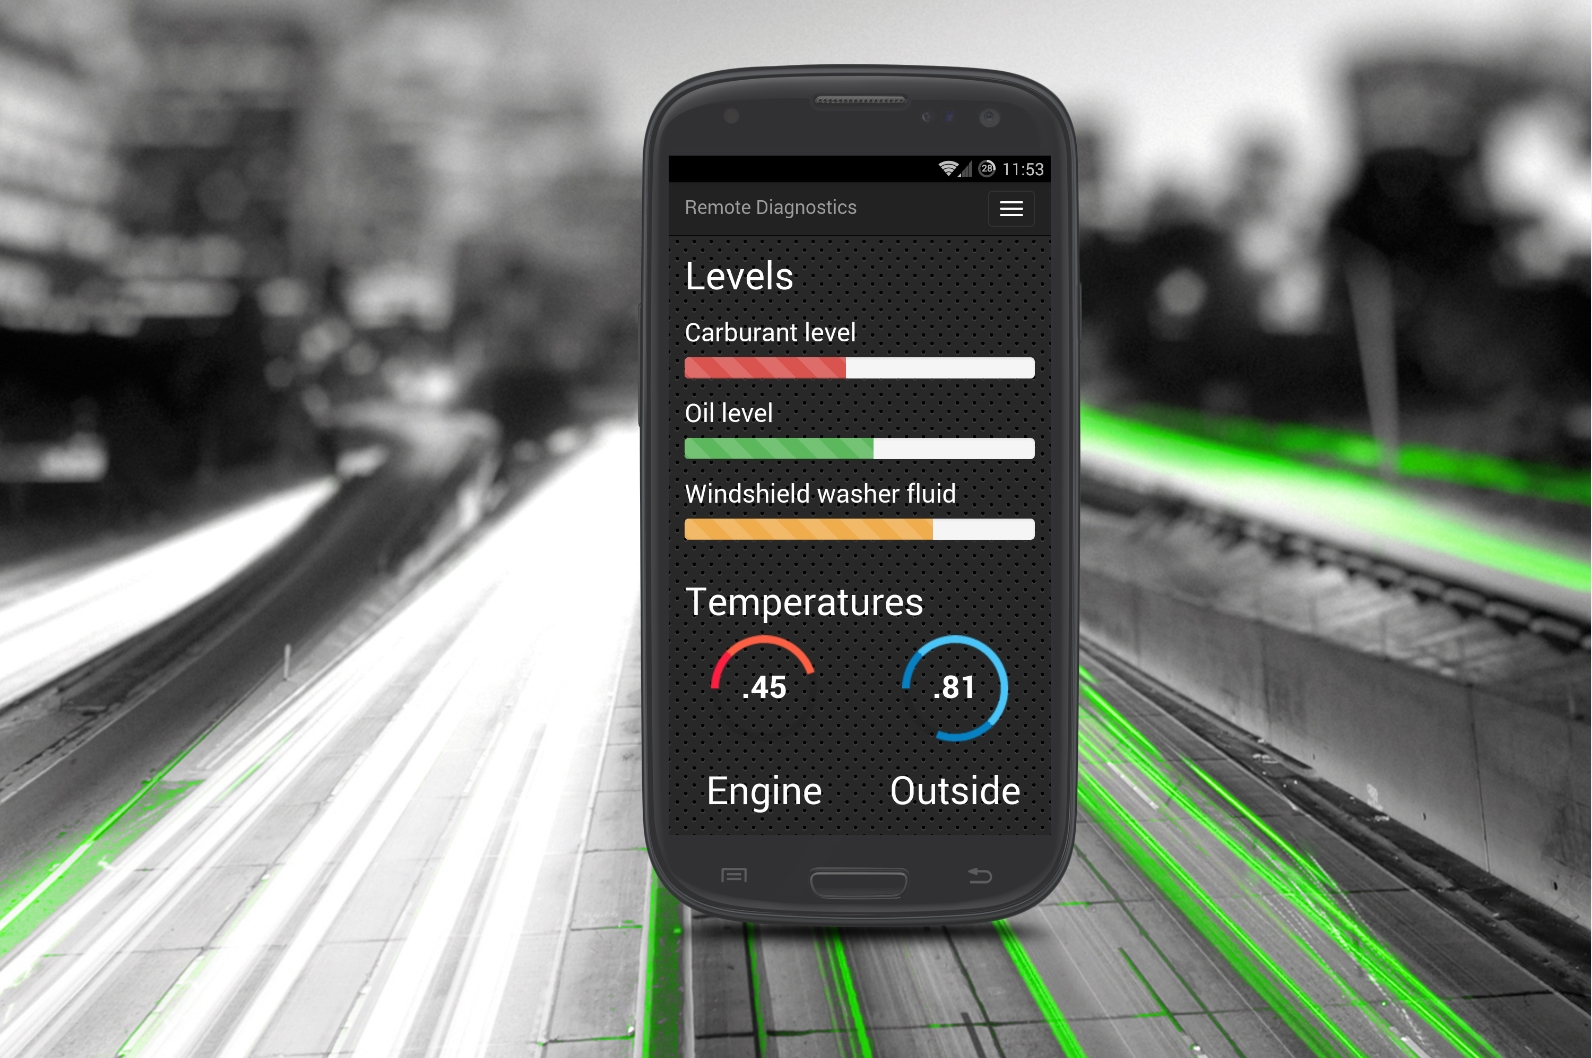
\includegraphics[width=1\textwidth]{./img/firstPage.jpg}
\end{figure}


\subsection{Keyboard Controller}
 
Through the Keyboard Controller one can control a RPi based car through Wi-Fi connection.
You just press the direction in which you want the car to go.
 
\begin{itemize}
\item REQ-1: Having some sort of direction controller for the steering of the car.
\end{itemize}
 
\begin{figure}[!htbp]
\center
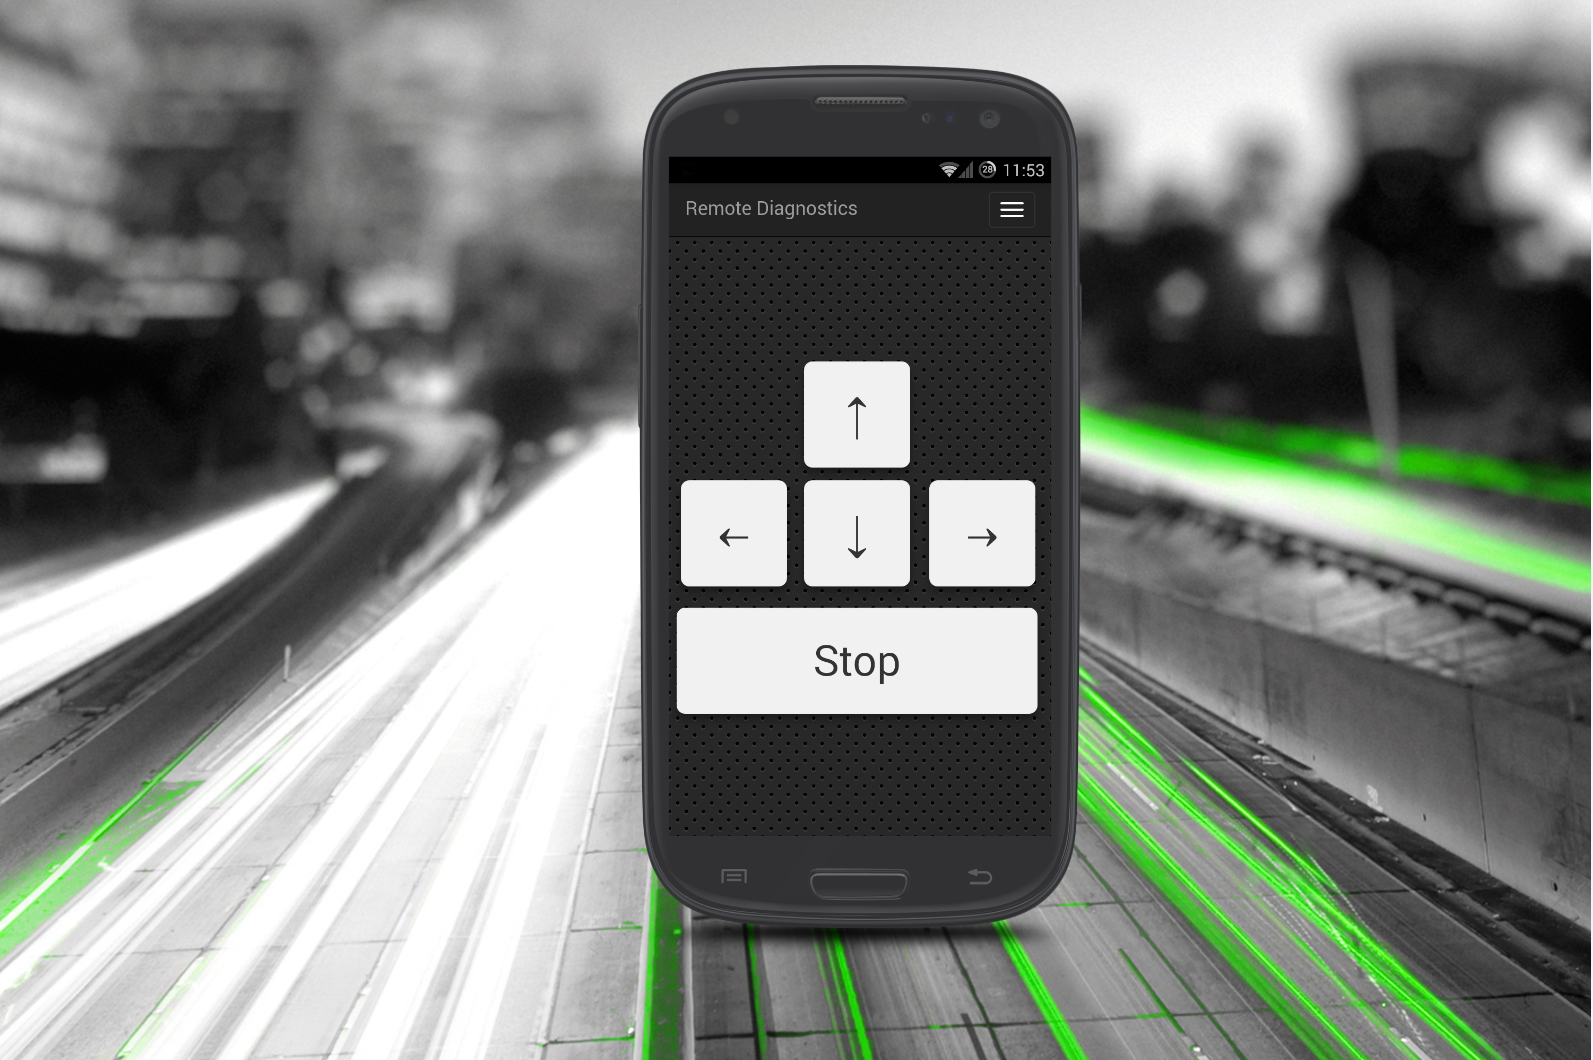
\includegraphics[width=1\textwidth]{./img/keyboardController.jpg}
Keyboard Controller
\end{figure}

\subsection{Gyroscope Controller}
You can also steer the car with the help of the gyroscope in another window.

\begin{itemize}
\item REQ-2: It is needed for the phone to have a gyroscope for controlling the car. 
\end{itemize}
 
\begin{figure}[!htbp]
\center
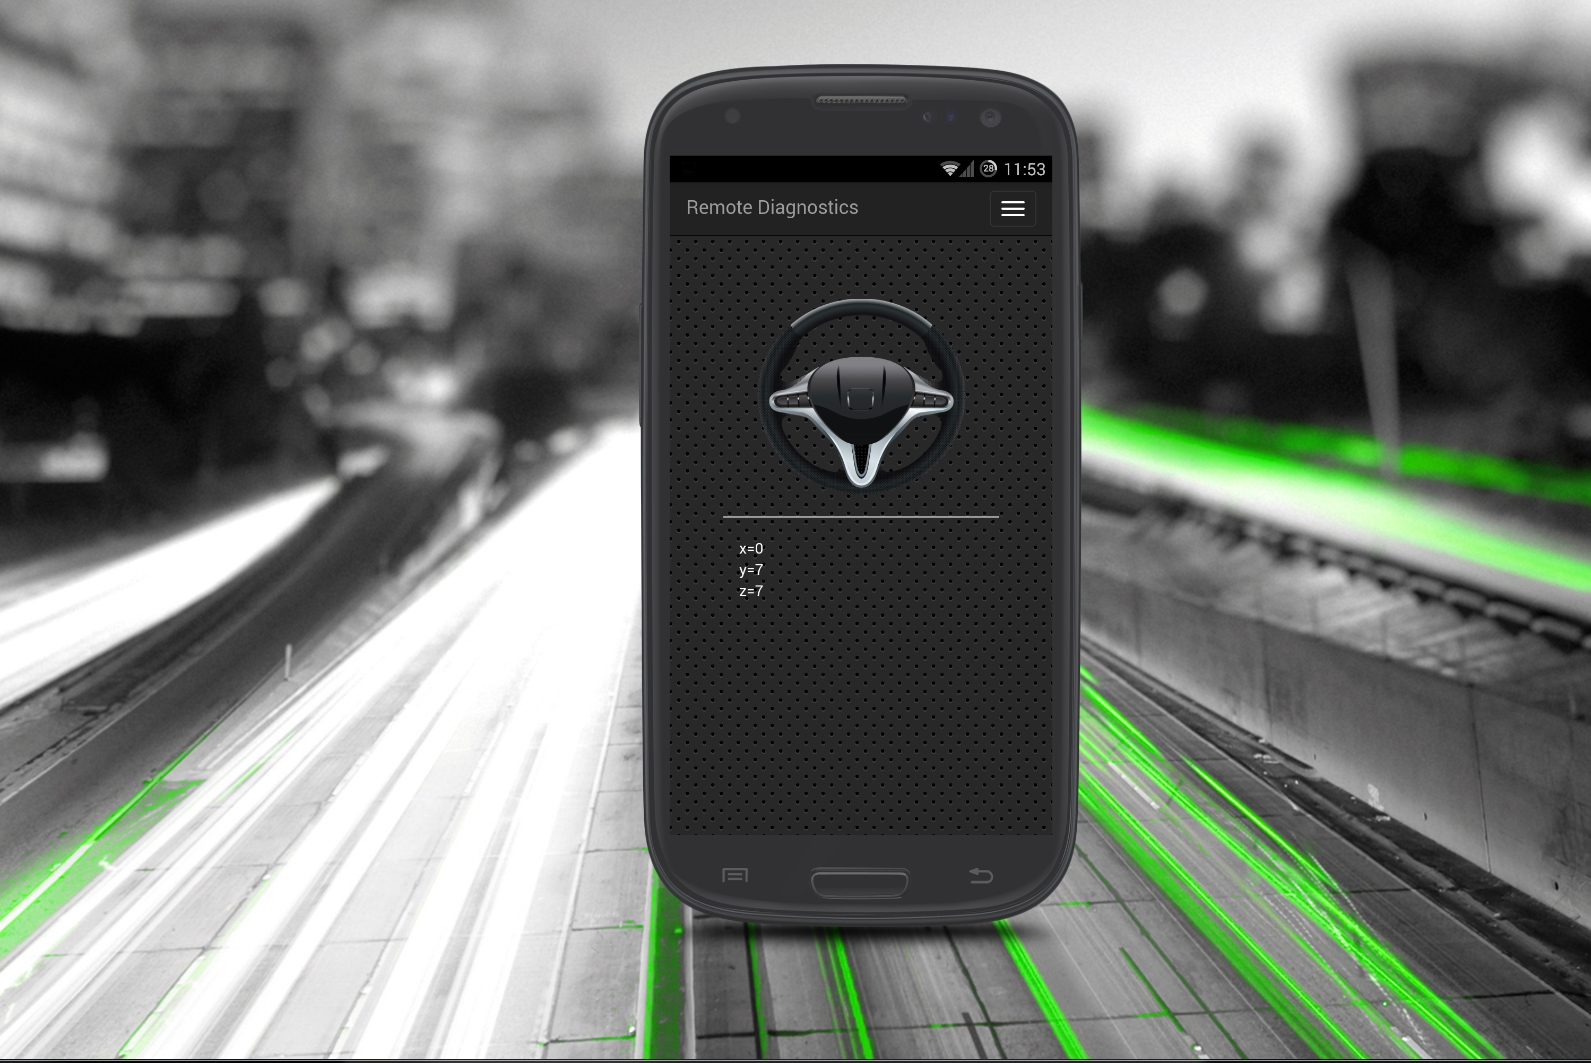
\includegraphics[width=1\textwidth]{./img/gyroController.jpg}
Gyroscope Controller
\end{figure}

\subsection{Speech Controller}
Through the phone's microphone you can give commands to the RPi controlled car. The commands are the following: forward, backwards, left, right, stop.
\begin{itemize}
\item REQ-3: It is needed for the phone to have a microphone for accepting voice messages.
\end{itemize}
\begin{figure}[!htbp]
\center
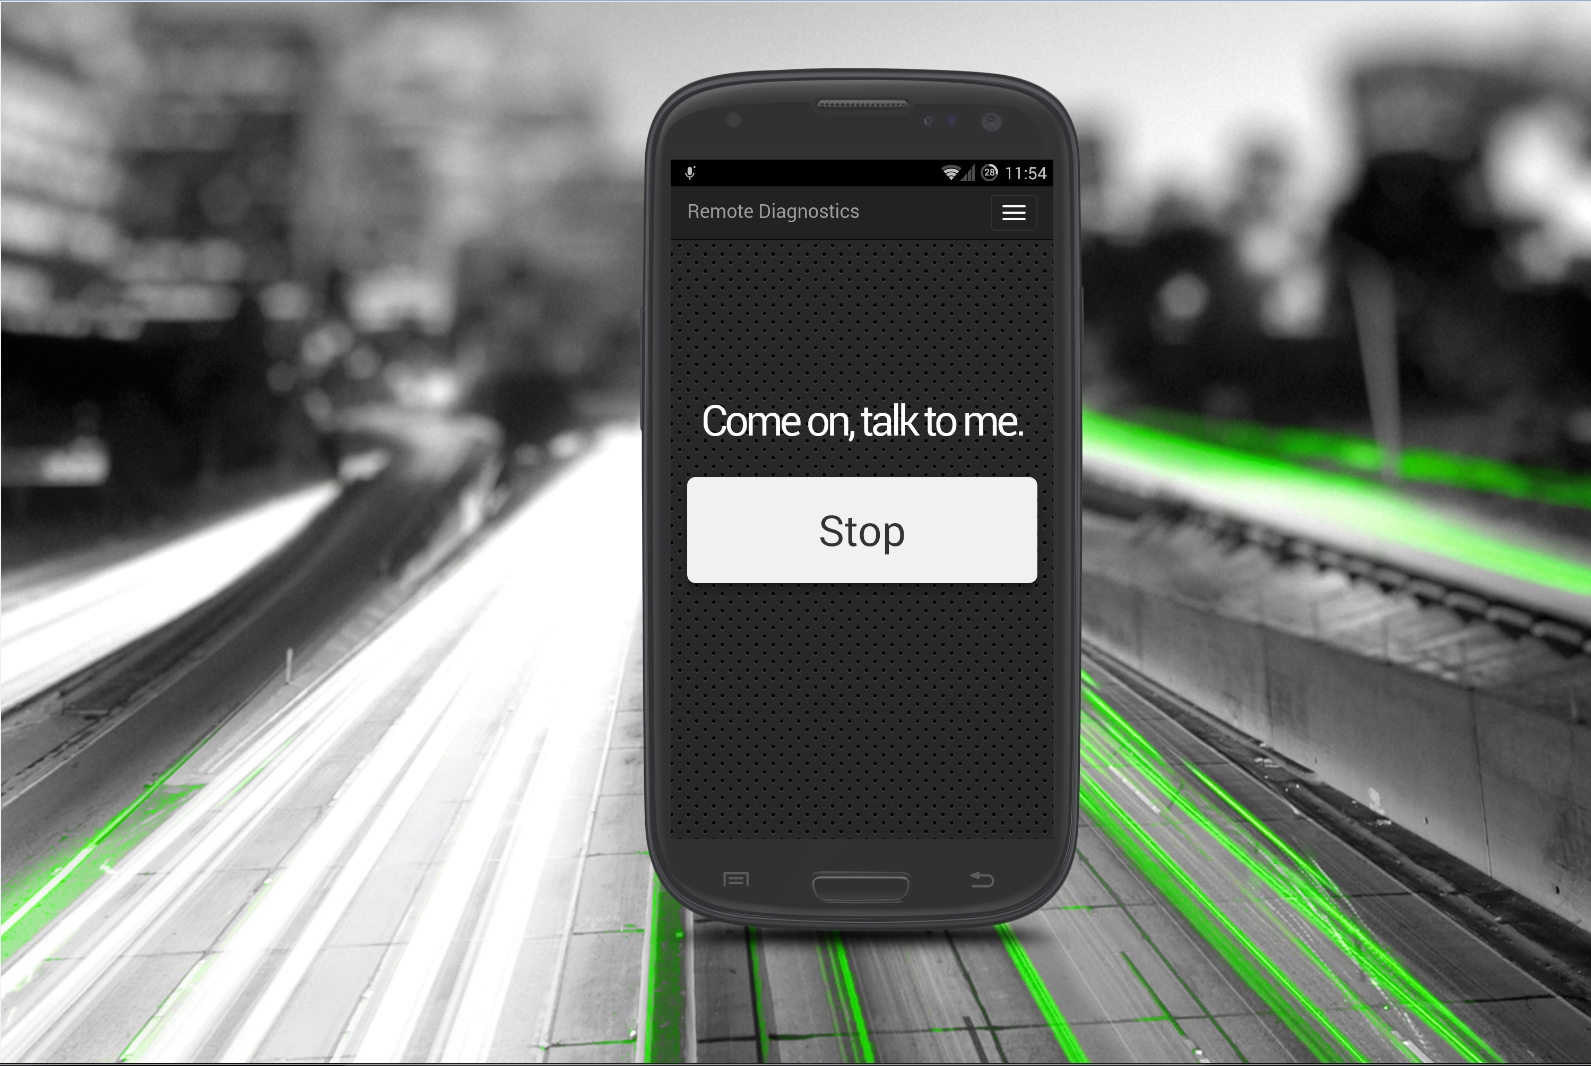
\includegraphics[width=1\textwidth]{./img/speechController.jpg}
Speech Controller
\end{figure}



\section{Hardware Interfaces}
There are three hardware pieces: 
\begin{itemize}
\item Phone
\item RaspberryPi
\item Car
\end{itemize}

The Raspberry Pi is bound to the car and it's connected to the same wifi network as the phone.
 

\section{Communications Interfaces}
The connection between the phone and the Raspberry is done through a Wi-Fi network. The application is on the web, so every communication is done through http.
\begin{itemize}
\item REQ-4 A good Wi-Fi connection is required for using the application.
\end{itemize}


\chapter{System Features}
This chapter illustrates organizing the functional requirements for the product by system features,
the major services provided by the product.


\section{Description and Priority}
This feature will retrieve the current sensor information from the ODB.
Retrieve sensor information is a High priority feature because it describes the core functionality of the system.

\section{Functional Requirements}
Safety requirements
\begin{itemize}
\item Description: Valid driving license for the user is needed
\item Rationale: You should not be able to control a car without knowing the current legislation laws and a basic training to control a car
\item Origin: The law
\item Fit criterion: Ensures the user stays alive
\item Dependencies: Having a valid driving license
\end{itemize}

\section{Limited car controlling capabilities}


\subsection{Description and Priority}
Limited car controlling capabilities is Low priority feature as the user can live without it.
This feature, although of low priority, has a high risk
rating in case of incindents produced by it (eg: car crash)


\chapter{Other Nonfunctional Requirements}

\section{Performance Requirements}
The system needs to be optimized for mobile usage.
As a general rule of thumb keep all page responses under 3 seconds in order
for the end-user not to get bored.

Keep everything as lightweight as possible in order to ensure that users with first generation smartphones
will also be able to use this software.

\begin{itemize}
\item REQ-5: System needs to be as optimized as possible so every user will be able to use it.
\end{itemize}
 

\section{Safety Requirements}
All users that wish to use the Limited car controlling capabilities feature must agree
that they are solely responsible for any possible loss, damage, or harm that could result from the use of this feature and must have
a valid driving's license.

\begin{itemize} 
\item REQ-6: Valid driving license for the user 
\end{itemize}

\part{Software Design Description}

\chapter{Use Cases}

\section{General use cases}
This is a usual use case just to check the state of the car.
\begin{figure}[!htb]
\center
\includegraphics[width=0.5\textwidth]{./uml/rmDiagGeneralUseCase.png}
\end{figure}

\section{Error message}
This is the case when the user receive an error message.
\begin{figure}[!htb]
\center
\includegraphics[width=1\textwidth]{./uml/rmDiagRemoteHelp.png}
\end{figure}

\begin{figure}[!htb]
\center
\includegraphics[width=1\textwidth]{./uml/rmDiagRemoteHelpActivity.png}
\end{figure}

\section{Components}
\begin{figure}[!htb]
\center
\includegraphics[width=1\textwidth]{./uml/swComponents.png}
\end{figure}
\newpage
\section{Controllers classes}
\begin{figure}[!htb]
\center
\includegraphics[width=1\textwidth]{./uml/controllers.png}
\end{figure}
\end{document}
